% Created 2022-03-07 Mon 16:46
% Intended LaTeX compiler: pdflatex
\documentclass[11pt]{article}
\usepackage[utf8]{inputenc}
\usepackage[T1]{fontenc}
\usepackage{graphicx}
\usepackage{grffile}
\usepackage{longtable}
\usepackage{wrapfig}
\usepackage{rotating}
\usepackage[normalem]{ulem}
\usepackage{amsmath}
\usepackage{textcomp}
\usepackage{amssymb}
\usepackage{capt-of}
\usepackage{hyperref}
\makeatletter
\newcommand{\citeprocitem}[2]{\hyper@linkstart{cite}{citeproc_bib_item_#1}#2\hyper@linkend}
\makeatother
\author{Adam Smith}
\date{\today}
\title{Thesis title}
\hypersetup{
 pdfauthor={Adam Smith},
 pdftitle={Thesis title},
 pdfkeywords={},
 pdfsubject={},
 pdfcreator={Emacs 27.2 (Org mode 9.4.4)}, 
 pdflang={English}}
\begin{document}

\maketitle
\begin{abstract}
This document shows you the syntax to type your thesis in latex or org-mode. It illustrates how to make footnotes, tables, equations and references to tables, equations etc.

If you want to work with latex only, look at the \texttt{.tex} file of this document. If you want to use emacs org-mode, then use the \texttt{.org} file. The pdf shows what the file looks like if you export it.

Running python code in this file only works in emacs org-mode; not in latex.
\end{abstract}

\newpage



\setcounter{tocdepth}{2}
\tableofcontents


\section{Introduction}
\label{sec:orgbab533a}
\label{sec:intro}

This file shows you how to use \href{https://www.gnu.org/software/emacs/}{emacs} \href{https://orgmode.org/}{org mode} to write a thesis. Shows you how to cite references, make footnotes, equations etc.

Alternatively, you can use latex directly in which case you can consider the file in this repository that ends in \texttt{.tex}.

In order to use emacs, you need to install it. The official website's download information: \url{https://www.gnu.org/software/emacs/download.html}

In Section \ref{sec:install} we explain how emacs can be installed.


\section{Literature references}
\label{sec:orgd785d69}

There are a number of ways in which you can do literature citations in org-mode. We will work with org-ref:
\begin{itemize}
\item \url{https://github.com/jkitchin/org-ref}
\end{itemize}

The syntax for including references is as follows. See Farrell and Klemperer \citeprocitem{2}{2007} for an analysis. We can also have references between brackets (\citeprocitem{1}{Athey and Imbens 2019}): that is, \texttt{citep} instead of \texttt{citet}. \texttt{armstrong-2007-chapt-coord} is the bibtex key, as you can see in the file \texttt{references.bib}.

If you use the \texttt{init.el} file for emacs, you can use the keys: C-c ] (press control (Ctrl) and c together; release these keys and then press the ]-key). The bottom part of the screen then gives you possible papers to cite from your \texttt{references.bib} file.


\section{Model}
\label{sec:orgf5f288e}

As we explained in section \ref{sec:intro}. This shows the syntax for a reference to a section, equation, table, figure etc. Type \texttt{ref:} and then the name of the label you are refering to. This can also be done with key strokes: C-c )

A label is typed in latex format as: \texttt{\textbackslash{}label\{name\_of\_label\}}. For org-mode you need to add \texttt{\#+name: name\_of\_label} to tables and figures.

Here we have some in-line math: \(x^2\).\footnote{This is a footnote.}

\begin{equation}
\label{eq:1}
a^2 + b^2 = c^2
\end{equation}

As we show in equation \eqref{eq:1}.

See Table \ref{table1}.

\begin{table}[htbp]
\caption{\label{tab:org243fa81}\label{table1} This table shows unemployment and gdp per head.}
\centering
\begin{tabular}{lrr}
country & unemployment & gdp\\
\hline
NL & 0.06 & 20000\\
UK & 0.01 & 19500\\
BE & 0.08 & 21100\\
\hline
average & 0.05 & 20200\\
\end{tabular}
\end{table}

Creating tables in org mode is a lot easier than in latex. Just type "|" name of column, another "|" name of second column, etc. end the line with "|", then press TAB.

If you want a horizontal line, type "|----" and press TAB.

In org mode (not in latex) you can add spreadsheet type calculations. See \url{https://orgmode.org/worg/org-tutorials/org-spreadsheet-intro.html} if you want to know more about this.


\begin{figure}[htbp]
\centering
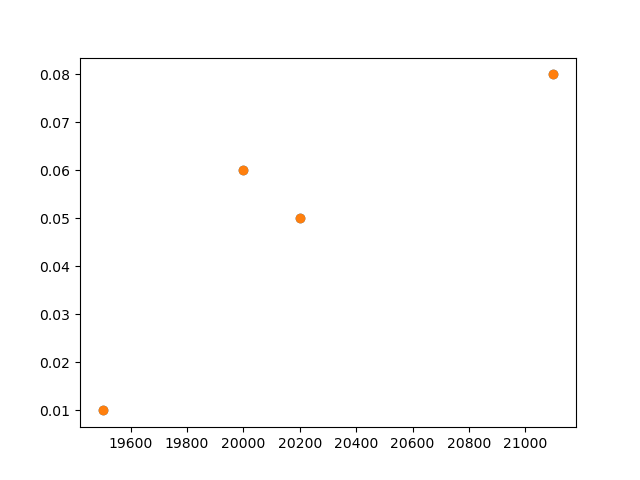
\includegraphics[width=.9\linewidth]{./fig.png}
\caption{\label{fig:org5acee25}\label{figure1} Figure with unemployment and gdp}
\end{figure}

See Figure \ref{figure1}.

\section{What should your editor be able to do?}
\label{sec:org8b1c9fe}

\subsection{Basics}
\label{sec:org9488e8c}

\begin{itemize}
\item type text\ldots{}
\item work on different parts of the same file in a split window
\item help with syntax, e.g. by providing snippets for equations, environments etc.
\begin{itemize}
\item e.g. with org cdlatex mode: type "equ" and then TAB to get an equation environment
\item ` a to get \(\alpha\)
\end{itemize}
\item operate on regions: e.g. for search and replace
\item operate on columns:
\begin{itemize}
\item delete columns in text
\item copy and past columns
\item add text in a column
\end{itemize}
\item add references to equations, sections, tables, figures
\item cite literature from a bibliography file
\item make it easy to add tables and edit tables (e.g. switch rows)
\item export to pdf
\end{itemize}

\subsection{Advanced}
\label{sec:orgdf7019f}

\begin{itemize}
\item combine code and latex
\item spreadsheet type capabilities
\item export to other formats, e.g. html
\end{itemize}


\subsubsection{why do we want to operate on columns?}
\label{sec:org531b277}

Turn the table here: \url{http://fmwww.bc.edu/ec-p/data/oecd/oecd.ctylist.html} into a python dictionary:
\begin{itemize}
\item C-v and block the start of each line
\item I and type '; then press ESC
\item block at the end of the abbreviation with C-v
\item type I and ' : '; then press ESC
\item block spaces (tab) to delete
\item block all lines with C-v
\item type \$ A ',; then press ESC
\item delete superfluous , at the end
\item add \{\} to turn this into a dictionary
\item a video on how to do this with regular emacs keybindings, can be found here: \url{https://www.youtube.com/watch?v=pcA5NeEudgU}
\end{itemize}

\begin{verbatim}
dict = {
'AUS' : 'Australia',
'AUT' : 'Austria',
'BEL' : 'Belgium',
'CAN' : 'Canada',
'CHE' : 'Switzerland',
'DEU' : 'Germany',
'DNK' : 'Denmark',
'ESP' : 'Spain',
'FIN' : 'Finland',
'FRA' : 'France',
'GBR' : 'Great Britain',
'GRC' : 'Greece',
'IRE' : 'Ireland',
'ISL' : 'Iceland',
'ITA' : 'Italy',
'JPN' : 'Japan',
'KOR' : 'South Korea',
'LUX' : 'Luxemburg',
'MEX' : 'Mexico',
'NLD' : 'Netherlands',
'NOR' : 'Norway',
'NZL' : 'New Zealand',
'PRT' : 'Portugal',
'SWE' : 'Sweden',
'TUR' : 'Turkey',
'USA' : 'United States'}
dict['NLD']
\end{verbatim}

Another trick we can use in org mode is to paste the table directly from the website:

AUS 	Australia
AUT 	Austria
BEL 	Belgium
CAN 	Canada
CHE 	Switzerland
DEU 	Germany
DNK 	Denmark
ESP 	Spain
FIN 	Finland
FRA 	France
GBR 	Great Britain
GRC 	Greece
IRE 	Ireland
ISL 	Iceland
ITA 	Italy
JPN 	Japan
KOR 	South Korea
LUX 	Luxemburg
MEX 	Mexico
NLD 	Netherlands
NOR 	Norway
NZL 	New Zealand
PRT 	Portugal
SWE 	Sweden
TUR 	Turkey
USA 	United States

\begin{itemize}
\item block the above table with Shift-V
\item M-x org-table-create-or-convert-from-region
\item and then add header with column names etc. to yield:
\end{itemize}

\begin{center}
\begin{tabular}{ll}
abbrev. & country name\\
\hline
AUS & Australia\\
AUT & Austria\\
BEL & Belgium\\
CAN & Canada\\
CHE & Switzerland\\
DEU & Germany\\
DNK & Denmark\\
ESP & Spain\\
FIN & Finland\\
FRA & France\\
GBR & Great Britain\\
GRC & Greece\\
IRE & Ireland\\
ISL & Iceland\\
ITA & Italy\\
JPN & Japan\\
KOR & South Korea\\
LUX & Luxemburg\\
MEX & Mexico\\
NLD & Netherlands\\
NOR & Norway\\
NZL & New Zealand\\
PRT & Portugal\\
SWE & Sweden\\
TUR & Turkey\\
USA & United States\\
\end{tabular}
\end{center}


\section{Conclusion}
\label{sec:org8064eda}

Here you can type the conclusion which is then followed by the bibliography.

\section{Bibliography}
\label{sec:org711c5e8}



\hypertarget{citeproc_bib_item_1}{Athey, Susan, and Guido W. Imbens. 2019. “Machine Learning Methods That Economists Should Know About.” \textit{Annual Review of Economics} 11 (1): 685–725. doi:\href{https://doi.org/10.1146/annurev-economics-080217-053433}{10.1146/annurev-economics-080217-053433}.}

\hypertarget{citeproc_bib_item_2}{Farrell, Joseph, and Paul Klemperer. 2007. “Chapter 31 Coordination and Lock-in: Competition with Switching Costs and Network Effects,” edited by M. Armstrong and R. Porter, 3:1967–2072. Handbook of Industrial Organization, Supplement C. Elsevier. doi:\href{https://doi.org/10.1016/S1573-448X(06)03031-7}{10.1016/S1573-448X(06)03031-7}.}





\newpage
\appendix


\section{Things to install}
\label{sec:org77fa432}
\label{sec:install}

\subsection{latex}
\label{sec:orgc7280e7}

Install latex: \url{https://www.latex-project.org/get/}



\subsection{latex editors if you do not want to use emacs}
\label{sec:org913afe0}

\begin{itemize}
\item winedt: \url{https://www.winedt.com/}
\item overleaf: \url{https://www.overleaf.com/}
\item texmaker: \url{https://www.xm1math.net/texmaker/}
\item tex studio: \url{https://www.texstudio.org/}
\end{itemize}

More general editors where you can also edit latex:

\begin{itemize}
\item atom: \url{https://atom.io/}
\begin{itemize}
\item and how to use with latex: \url{https://towardsdatascience.com/setting-up-latex-on-your-atom-editor-7ea624571d50}
\end{itemize}
\item vim: \url{https://www.vim.org/docs.php}
\end{itemize}


\subsection{git}
\label{sec:orged07eba}

install git: \url{https://git-scm.com/downloads}

\subsection{Emacs}
\label{sec:org7a8a5fc}

In the lecture I will illustrate what an editor can/should do using emacs.


\subsubsection{Emacs on Windows}
\label{sec:orgc43b2b5}

\begin{itemize}
\item go to: \url{http://mirror.team-cymru.com/gnu/emacs/windows/emacs-27/}
\item download emacs-27.2-x86\textsubscript{64}-installer.exe to your Downloads folder: \url{http://mirror.team-cymru.com/gnu/emacs/windows/emacs-27/emacs-27.2-x86\_64-installer.exe}
\item run the downloaded \texttt{exe} file
\end{itemize}

\subsubsection{Emacs on Mac OS}
\label{sec:org028ce58}

For Mac Os:
\begin{itemize}
\item install homebrew: \url{https://brew.sh/}
\end{itemize}

Open a terminal and type the following lines:

\begin{verbatim}
brew tap d12frosted/emacs-plus
brew install emacs-plus
\end{verbatim}

\subsubsection{Emacs on Linux}
\label{sec:org71c0495}

When you are using Linux, you probably know what you are doing. But just in case, the commands for your package manager can be found here: \url{https://www.gnu.org/software/emacs/download.html}


\subsubsection{org-mode}
\label{sec:org9bbf7d6}

When you install emacs, org-mode is installed as well (comes with emacs)


\subsection{introductions to emacs}
\label{sec:org545ac6b}

It is easy to get lost in emacs. Hence do not try to use everything at once. A couple of basic things, you need from the start (like opening and saving files). For the other things: move step-by-step. 

A great starting point, explaining key-bindings etc. is:
\begin{itemize}
\item \url{https://systemcrafters.net/emacs-essentials/absolute-beginners-guide-to-emacs/}
\begin{itemize}
\item and the video that goes with it: \url{https://www.youtube.com/watch?v=48JlgiBpw\_I}
\item this explains things like "M-x", "C-c", "C-x" etc. which you can see when you use menu items like "file"
\begin{itemize}
\item to illustrate, use your mouse to click on "File" in the top left corner
\item the first item is: "Visit New File\ldots{} C-x C-f"
\item you can click on this item to open a file; but you can also use the key combination C-x C-f which means: press Control (Ctrl) and x together; release these keys; then press Ctrl and f together. This allows you to open a file. If you type the name of a file that does not exist yet, this new file will be created
\item you save a file with C-x C-s; hence you can quickly save a file by pressing these keys without having to reach for the mouse
\item the emacs configuration below helps as it uses the which-key package. After typing C-x, it shows you what other keys you can use.
\end{itemize}
\end{itemize}
\end{itemize}

There are other great introductions to emacs as well:
\begin{itemize}
\item \url{https://www.youtube.com/playlist?list=PL9KxKa8NpFxIcNQa9js7dQQIHc81b0-Xg}
\item \url{https://www.youtube.com/playlist?list=PLwTHcico4iPMlBZPin6catRcUDzf7NNVs}
\item or google emacs tutorial or emacs for beginners
\item finally, emacs is self documenting: all information can be found in emacs as well, just type C-h i
\begin{itemize}
\item this gives information on emacs and all the packages you installed with emacs
\end{itemize}
\end{itemize}


\subsection{next steps}
\label{sec:orgf3c3a43}

You can extend the configuration of emacs by yourself, e.g. by watching tutorials like: \url{https://www.youtube.com/playlist?list=PLEoMzSkcN8oNmd98m\_6FoaJseUsa6QGm2}

Or you can use pre-configured emacs distributions like scimax and doom emacs.


\subsubsection{scimax}
\label{sec:orgdff1aaa}

Scimax is developed for engineers, but works perfectly well for economists. More details can be found here:
\begin{itemize}
\item \url{https://github.com/jkitchin/scimax}
\item youtube playlist with scimax features: \url{https://www.youtube.com/playlist?list=PL0sMmOaE\_gs3E0OjExoI7vlCAVygj6S4I}
\end{itemize}

\subsubsection{Doom}
\label{sec:org4ab38dd}

Emacs has an absurd number of features and how do you choose the right ones if you do not know about them? Doom emacs has very reasonable default settings:
\begin{itemize}
\item \url{https://github.com/hlissner/doom-emacs}
\item Doom emacs for noobs: \url{https://www.youtube.com/watch?v=iab2z21cRqA}
\item Doom emacs getting started: \url{https://www.youtube.com/watch?v=dr\_iBj91eeI}
\item youtube playlist: \url{https://www.youtube.com/playlist?list=PLhXZp00uXBk4np17N39WvB80zgxlZfVwj}
\end{itemize}
\end{document}